\subsection{Testing scenarios}
In order to prepare the WLCG infrastructure for IPv6, the best
approach is to identify beforehand the relevant use cases, starting
from the simplest ones, to take into account the likely constraints
from sites and finally to define realistic scenarios to be used for
testing.

It is reasonable to assume that all central services must work in
dual-stack mode, to be compatible with both IPv4 and IPv6
clients. Site services are strongly encouraged to be run in dual stack
mode as well, lest they incur in limitations (for example in joining
storage federations). On the other hand, clients (including users,
software agents and jobs running on worker nodes) should be able to
exclusively use either protocol: users may connect from arbitrary
nodes (e.g. their laptops) while compute nodes at some sites might have
only IPv6 public addresses.

To summarise, any testing should comply with these requirements:
\begin{itemize}
\item all services must be tested in dual stack
\item all user clients must be tested in IPv4 and dual stack
\item all batch nodes must be tested in IPv4, IPv6 and dual stack (not all configurations might be possible for a given site)
\end{itemize}

The use cases to test are of increasing complexity and should be addressed in this order:
\begin{enumerate}[a.]
\item basic job submission, either direct (via CREAM client \cite{cream}, Condor-G, etc.) or via workload management services (EMI WMS \cite{wms}, glideinWMS, PanDA \cite{panda}, etc.)
\item basic data transfer from/to a user node to/from a storage element
\item third party data transfer (e.g. via FTS \cite{fts})
\item production data transfer (e.g. via PhEDEX \cite{phedgen}, DIRAC, etc.)
\item conditions data access (e.g. via Frontier/squid)
\item experiment software access (e.g. via CVMFS \cite{cvmfs})
\item experiment workflow, running a complete production/analysis task
\item information system query (e.g. via BDII \cite{bdii})
\item job monitoring (e.g. via MonALISA \cite{monalisa}, experiment dashboards, etc.)
\end{enumerate}
In all cases, all relevant client/service combinations in terms of network protocols should be addressed. For simplicity, ``auxiliary'' services (ARGUS, VOMS, MYProxy, etc.) running only IPv4 may be used.


\subsection{Point-to-point testing}

We used the PhEDEx LifeCycle agent \cite{LifeCycle} to drive transfers between pairs of sites, using gridftp with the IPv6 connectivity flags. Filesizes were checked at the destination, and any failures recorded. Files were transferred in both directions between each site pair.

Initially, we simply tested connectivity and basic functionality. We also tested under specific conditions, e.g. to compare throughput and error rates with IPv6 vs. IPv4 connectivity. This was useful for debugging issues with firewalls, etc.

Since March 2013 the transfer testbed is running continuously, with more sites joining over time. Finally we have 12 sites transferring 1 GB files among each other.

To date, we have transferred over 2 PB of data between the 12 sites over the 6 months since the testbed started continuous operations. This is 7\% of the rate that CMS \cite{cms} achieve in daily operations, so is quite significant. The average success rate is 87\%, which is very high considering that the testbed is operated at-risk. Errors are only detected when someone decides to look for them, and were often left unfixed to aid debugging.
So we can conclude that gridftp transfers over IPv6 are very reliable, given adequate hardware to run on.

Figure \ref{fig:full-mesh} shows transfer results for the full mesh of sites. The source site is shown along the rows, the destination site is shown in the columns. All plots are scaled to an x-axis of 500 seconds (corresponding to a transfer rate of 2 MB/sec), and only successful transfers are shown.

We can see that, in general, transfers were fast, the graphs mostly peak to the left. Some sites (IHEP Beijing, Chicago) have long tails for transfers out, though transfers to them are more successful.

\subsection{Testing with PhEDEx transfers}
We also tested with PhEDEx (\cite{PhEDEx}), the CMS data-placement system. We used two WLCG/GridPP sites (Imperial College London and Glasgow) with IPv6-enabled Disk Pool Manager (DPM) storage elements, and transfers via a dual-stack FTS3 (\cite{FTS3}) server at Imperial College. Transfers were throttled to limit the load on the servers, and have been running smoothly for nearly two months at the time of writing, transferring over 120 TB of data. This tells us that PhEDEx can indeed operate to CMS production standards with IPv6-enabled services.
% Figure \ref{fig:phedex-transfer-volume} shows the accumulated volume of data transferred from mid-August until early October 2013, by which point over 120 TB of data had been transferred with very few errors. This tells us that PhEDEx can indeed operate to CMS production standards with IPv6-enabled services.

% To create this graphic:
% 1) save your image as a 1024x1024 png/gif/bmp
% 2) convert to pdf (install ImageMagick, then 'convert FileIn.png FileOut.pdf')
% 3) to resize the image, if needed, 'convert FileIn.png -resize 66% FileOut.pdf' etc
% N.B. if the input and output files have the same base name, LaTeX will prefer to take the png
% over the pdf, which is probably not what you want. Make sure the files have different names!
\begin{figure}[htp]
\centering
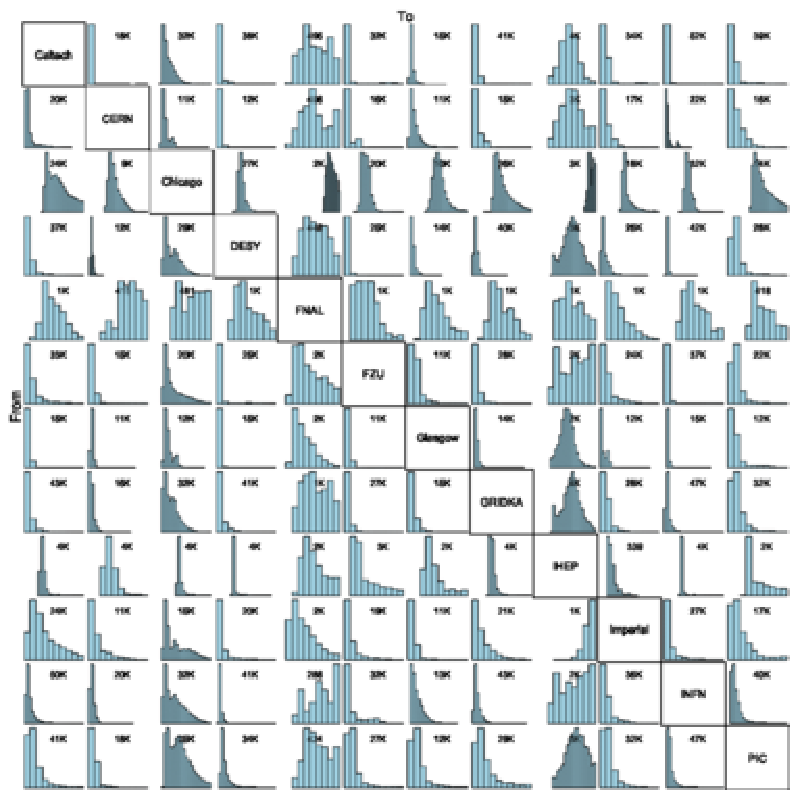
\includegraphics{full-mesh}
\caption{Transfer performance for the IPv6 testbed continuous transfers. A 1 GB file is transferred between each pair of sites, then deleted, then transferred again, continuously. The plots show the distribution of transfer duration times per site pair. The source site is named in the row, the destination site is named in the column. So the top-right plot shows transfers from Caltech to PIC, the bottom-left shows transfers from PIC to Caltech. The x-axis is in seconds, from 0 to 500 for each plot. The number inset in each plot shows the approximate number of transfers between that site pair in that direction.}\label{fig:full-mesh}
\end{figure}

%\begin{figure}[htp]
%\centering
%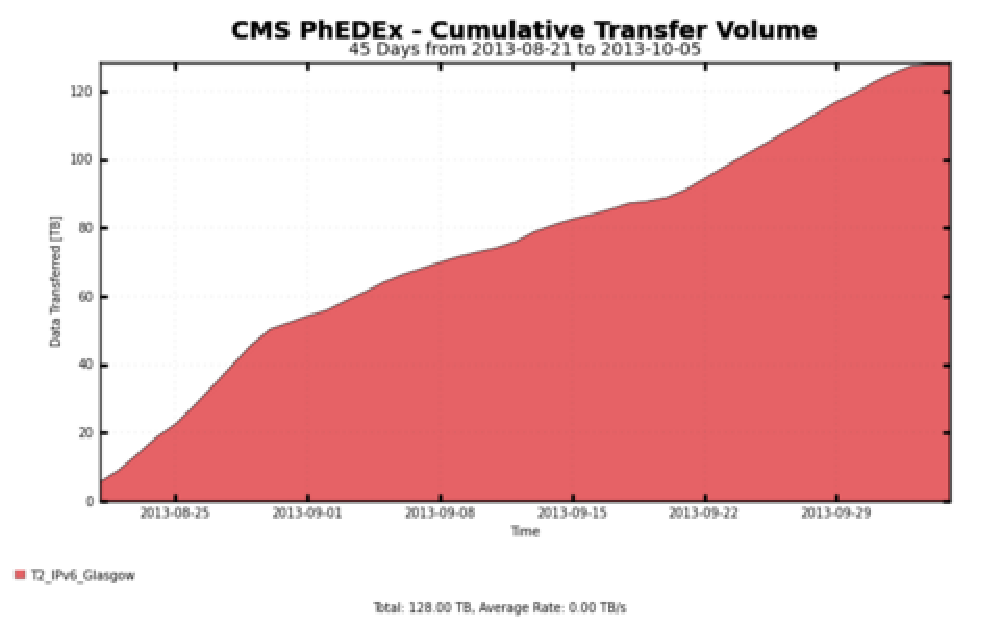
\includegraphics{phedex-transfer-volume}
%\caption{Cumulative data-transfer between Imperial College and Glasgow using PhEDEx on the IPv6 testbed.}\label{fig:phedex-transfer-volume}
%\end{figure}

\subsection{Dual-stack hosts at Imperial College London}
The WLCG/GridPP site within the HEP group at Imperial College London (UKI-LT2-IC-HEP) has configured a subset of its hosts to be dual-stack. 
The site currently runs dual-stack DNS, SSH, NFS, EMI 2 and EMI 3 CREAM CEs, EMI 2 Worker Nodes, 
ARC CE and dCache (headnode, SRM component only) services.
Additionally, all BDII services including top and site BDIIs run in dual-stack mode. The Puppet configuration system and the local OS install system have been left IPv4-only.
This set up was achieved in a number of stages. Initially, the local campus network team enabled 
stateless address autoconfiguration (SLAAC) on the subnet routers servicing the grid hosts. {\em All hosts} acquired an IPv6 address via autoconfiguration. 
No subsequent problems were observed and no hosts required IPv6 to be turned off in order to continue normal operations. 
Next, AAAA records were added to core services such as mail and LDAP. The DNS servers had static IPv6 addresses added. 
The IPv6 DNS server hostnames were added into {\tt /etc/resolv.conf} on all hosts. AAAA and PTR records were added to the worker nodes and these were made to point to the SLAAC addresses. 
On relevant service hosts the IPv6 firewall was configured as appropriate. On hosts running a BDII service the IPv6 option was enabled explicitly 
(by setting {\tt BDII\_IPV6\_SUPPORT=yes} in {\tt /etc/sysconfig/bdii}).
